% Snowflake Data Engineering — Chapter 5 | original manuscript draft
% Author: Arman Golbidi | Editorial snapshot: 22 October 2026
% Compile: xelatex -interaction=nonstopmode -halt-on-error Snowflake_Data_Engineering_Chapter_05.tex
% Trim: 178 x 254 mm; margins inside 23 mm / outside 17 mm / top-bottom 19 mm.
% Body: 10.75 pt / 13.65 pt leading = 1.27 line-height ratio; code: 8.75 pt.
\documentclass[11pt,twoside]{article}
\usepackage[paperwidth=178mm,paperheight=254mm,inner=23mm,outer=17mm,top=19mm,bottom=19mm,headheight=5mm,headsep=4mm,footskip=9mm]{geometry}
\usepackage{fontspec}
\setmainfont{LibertinusSerif-Regular.otf}[BoldFont=LibertinusSerif-Bold.otf,ItalicFont=LibertinusSerif-Italic.otf,BoldItalicFont=LibertinusSerif-BoldItalic.otf]
\setsansfont{LibertinusSans-Regular.otf}[BoldFont=LibertinusSans-Bold.otf,ItalicFont=LibertinusSans-Italic.otf]
\setmonofont{LibertinusMono-Regular.otf}[Scale=0.91]
\usepackage[english]{babel}
\usepackage{microtype}
\usepackage{setspace}
\setstretch{1.0}
\usepackage{titlesec,enumitem,tabularx,array,booktabs,needspace,fancyhdr,lastpage}
\usepackage[most]{tcolorbox}
\usepackage{tikz}
\usetikzlibrary{arrows.meta,positioning,fit,shapes.misc,calc}
\usepackage{listings}
\usepackage{xcolor}
\usepackage{hyperref}
\usepackage{amsmath}
\hypersetup{colorlinks=true,urlcolor=steelblue,linkcolor=steelblue,pdfauthor={Arman Golbidi},pdftitle={Snowflake Data Engineering - Chapter 5: Batch Data Ingestion and Loading},pdfsubject={English technical book manuscript, fourth chapter, 178 x 254 mm}}
\definecolor{navy}{HTML}{15334A}
\definecolor{steelblue}{HTML}{17779B}
\definecolor{teal}{HTML}{12888A}
\definecolor{lightblue}{HTML}{ECF5F7}
\definecolor{papergray}{HTML}{F2F5F6}
\definecolor{inkgray}{HTML}{4A5862}
\definecolor{thinrule}{HTML}{CBD7DB}
\AtBeginDocument{\color{navy}\fontsize{10.75}{13.65}\selectfont}
\setlength{\parindent}{0pt}
\emergencystretch=1.3em
\setlength{\parskip}{3.3pt plus 0.7pt minus 0.6pt}
\setlist[itemize]{leftmargin=4mm,itemsep=1pt,topsep=2pt,parsep=0pt}
\setlist[enumerate]{leftmargin=5mm,itemsep=1pt,topsep=2pt}
\titleformat{\section}{\sffamily\bfseries\color{navy}\fontsize{14}{17}\selectfont}{}{0pt}{}
\titlespacing*{\section}{0pt}{8pt}{4pt}
\titleformat{\subsection}{\sffamily\bfseries\color{steelblue}\fontsize{10.8}{13}\selectfont}{}{0pt}{}
\titlespacing*{\subsection}{0pt}{5pt}{1pt}
\newcommand{\topic}[2]{\subsection*{#1\quad #2}}
\newcommand{\repo}[2]{\par\begingroup\fontsize{8.0}{9.6}\selectfont\sffamily\color{inkgray}\textbf{Project reference:} \href{#2}{#1}. \textit{Not independently executed; rights review pending.}\par\endgroup}
\newtcolorbox{insight}[1][]{enhanced,breakable,colback=lightblue,colframe=thinrule,boxrule=.45pt,arc=1.3mm,left=2.8mm,right=2.8mm,top=1.8mm,bottom=1.8mm,before skip=5pt,after skip=5pt,#1}
\newtcolorbox{whitebox}[1][]{enhanced,breakable,colback=papergray,colframe=thinrule,boxrule=.35pt,arc=1mm,left=2.6mm,right=2.6mm,top=1.5mm,bottom=1.5mm,before skip=4pt,after skip=5pt,#1}
\lstdefinestyle{chaptercode}{basicstyle=\ttfamily\fontsize{8.75}{10.7}\selectfont,backgroundcolor=\color{papergray},frame=single,framerule=.35pt,rulecolor=\color{thinrule},breaklines=true,columns=fullflexible,keepspaces=true,showstringspaces=false,aboveskip=5pt,belowskip=5pt,xleftmargin=2mm,xrightmargin=1mm,framexleftmargin=2mm,framexrightmargin=1mm}
\lstset{style=chaptercode}
\pagestyle{fancy}
\fancyhf{}
\fancyhead[LE]{\sffamily\fontsize{7.6}{9}\selectfont\color{inkgray}\textsc{Snowflake Data Engineering}}
\fancyhead[RO]{\sffamily\fontsize{7.6}{9}\selectfont\color{inkgray}\textsc{05 / Batch Data Ingestion}}
\fancyfoot[LE,RO]{\sffamily\bfseries\fontsize{8.2}{9}\selectfont\color{steelblue}\thepage}
\fancyfoot[LO,RE]{\sffamily\fontsize{7.6}{9}\selectfont\color{inkgray}Arman Golbidi \quad | \quad Chapter 05}
\renewcommand{\headrulewidth}{0.35pt}
\renewcommand{\footrulewidth}{0pt}
\setcounter{page}{77}
\raggedbottom

% CHAPTER 04 ONLY, pages 77--96 in the planned book
\begin{document}
% ------------------------------------------------------------------------
% CHAPTER 05. Individual physical pages are delimited to preserve 20-page plan.
% ------------------------------------------------------------------------
% page 77 / chapter opening
{\sffamily\bfseries\fontsize{9}{11}\selectfont\color{steelblue} CHAPTER 05 \hfill DATA ENGINEERING / INGESTION}\par\vspace{4mm}
{\sffamily\bfseries\fontsize{23}{27}\selectfont\color{navy} Batch Data Ingestion\\and Loading}\par\vspace{3mm}
{\sffamily\fontsize{11.4}{14}\selectfont\color{steelblue} From trustworthy source files to an auditable bronze layer}\par\vspace{7mm}
\begin{insight}\textbf{A plausible number is not necessarily a trustworthy number.}\par
An energy analyst opens Monday's dashboard and notices that Finnish electricity generation has apparently increased by 14 percent overnight. A colleague celebrates; another asks whether the meter network changed. The actual cause is less exciting: Sunday's CSV file was loaded twice after a failed scheduler retry. Nothing crashed. Every SQL statement succeeded. The pipeline was wrong.\end{insight}
Loading is not merely a file transfer. The warehouse must reconcile a publisher's export, preserved bytes, loaded rows, and the observations safe to count. An engineer preserves the evidence connecting them.

We build the ingestion boundary for the \emph{Finland Energy Analytics} project from Chapters~1 and~4. A public dataset does not automatically permit republication, so the initial fixture is explicitly \emph{synthetic}. Real Finnish data require separate rights, schema and provenance checks.

\begin{whitebox}\textbf{By the end of this chapter, you can:}
\begin{itemize}
\item specify source contracts, freshness and licensing checks before writing a loader;
\item select file formats, stages and safe Snowflake \texttt{COPY INTO} settings;
\item retain file and row provenance, reject bad input, and reconcile a batch;
\item explain what duplicate-file prevention does \emph{not} guarantee;
\item prepare a repeatable Python-assisted transfer, monitoring and recovery plan.
\end{itemize}\end{whitebox}
\textbf{Prerequisites.} Chapters~3--4, elementary SQL and optional Python~3. A real Snowflake lab requires an authorized account, role with object privileges, and a small virtual warehouse. An offline validation path is provided in the companion materials. None of the example outputs below is presented as a measured cloud benchmark.

\begin{center}
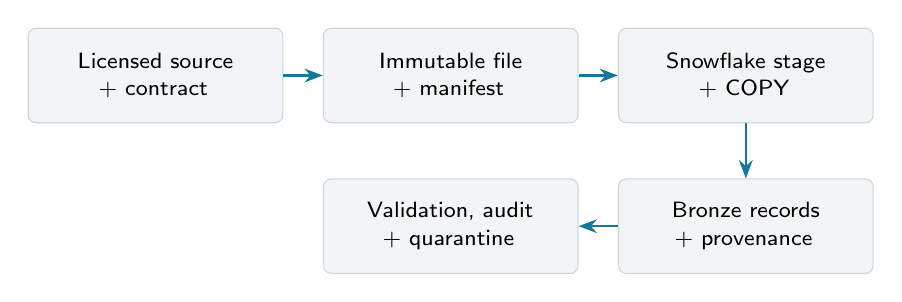
\begin{tikzpicture}[>=Stealth,node distance=5mm, every node/.style={font=\sffamily\fontsize{8.1}{10}\selectfont},bx/.style={draw=thinrule,rounded corners=1mm,fill=papergray,align=center,minimum height=12mm,text width=30mm}]
\node[bx] (a) {Licensed source\\+ contract};
\node[bx,right=of a] (b) {Immutable file\\+ manifest};
\node[bx,right=of b] (c) {Snowflake stage\\+ COPY};
\node[bx,below=7mm of c] (d) {Bronze records\\+ provenance};
\node[bx,left=of d] (e) {Validation, audit\\+ quarantine};
\draw[->,thick,steelblue](a)--(b);\draw[->,thick,steelblue](b)--(c);\draw[->,thick,steelblue](c)--(d);\draw[->,thick,steelblue](d)--(e);
\end{tikzpicture}\par{\fontsize{8}{10}\selectfont\color{inkgray}Figure 5.1. The ingestion boundary preserves both data and evidence.}\end{center}
\newpage
% page 78
\section*{5.1\quad Data source assessment and ingestion requirements}
\topic{5.1.1}{Source endpoints, formats, and refresh intervals}
Before choosing between a Python script and a managed connector, build a \emph{source inventory}. At minimum, record the publisher, access method (HTTPS API, SFTP, database export or cloud bucket), file format, date/time semantics, grain, expected size, nominal cadence, revision policy and a human contact. The source inventory is a technical contract with your future self: it tells you what to investigate when yesterday's source files stop looking like today's.

A useful distinction is between \emph{publication time}, when a source claims to have released a revision; \emph{event time}, when an observation actually occurred; and \emph{ingestion time}, when your platform received it. These clocks are not interchangeable. A monthly correction published today can legitimately update a measurement from the previous year. If you partition only by ingestion date, such late-arriving corrections still need a business-key reconciliation.

\begin{center}\small\begin{tabularx}{\linewidth}{@{}>{\bfseries}p{33mm}X@{}}\toprule
Contract field & Example / decision for a synthetic energy source\\\midrule
Source identifier & \texttt{fi\_energy\_demo}; accountable source owner\\
Primary access & HTTPS batch download or reviewed local fixture\\
Payload & UTF-8 CSV, comma delimiter, one header row\\
Observation grain & source + metric + UTC interval start\\
Publication cadence & Hourly export, checked daily (illustrative)\\
Correction rule & Same business key may be republished with revision\\
Required evidence & URL, retrieval time, license, SHA-256, row count\\\bottomrule\end{tabularx}\end{center}
An endpoint can remain reachable while delivering stale content. Conversely, an HTTP timeout does not establish that the publisher has no new data. Treat access success and dataset freshness as separate health checks. In file-based systems, the \emph{inventory} should also capture whether a batch is a complete snapshot, a changed-row extract or a sequence of disjoint partitions; the recovery process depends on that meaning.

\textbf{Design decision.} For the book's first runnable load, prefer two small immutable CSV files. A reader can inspect their bytes, calculate expected rows by hand, and reason about retries. The later streaming chapter will address cases where files cannot meet the service objective.

\repo{P046: Snowflake Google Analytics connector guide}{https://github.com/Snowflake-Labs/sfguide-getting-started-with-snowflake-connector-for-google-analytics}
\newpage
% page 79
\topic{5.1.2}{Availability, API quota, and dataset licensing}
Public accessibility is not the same as legal permission to republish a dataset. A responsible ingestion design records where the data comes from, its permitted uses, attribution conditions, retention restrictions and whether redistribution in a commercial technical book is allowed. A direct public URL is evidence of discoverability; it is \emph{not} proof of a reusable license. For a Finnish energy source, preserve a dated copy of the source's own terms and link to the official publisher. Do not infer permissions from generic national open-data policies.

API constraints belong in the same review. Record authentication, per-minute or daily quotas, pagination, maximum response size, support for conditional requests, changes to endpoints, and how HTTP status codes are used. Never retry a permanent authorization failure as though it were a transient outage. For retryable failures such as temporary throttling, honor \texttt{Retry-After} when present, use bounded exponential backoff and cap the total retry duration.

\begin{whitebox}\textbf{Source admission checklist}\par
\begin{enumerate}
\item \textbf{Legal and ethical:} dataset rights, personal-data exposure, appropriate attribution and acceptable use.
\item \textbf{Operational:} uptime assumptions, rate limit, payload pagination, contact and incident channel.
\item \textbf{Semantic:} units, time zone, revisions, missing intervals, negative values and category definitions.
\item \textbf{Audit:} stable source ID, retrieval log, checksum, immutable archive and manifest.
\end{enumerate}\end{whitebox}
An unreliable publisher may still be useful if the consumer can tolerate a larger freshness window and an explicit ``data delayed'' state. A high-value dashboard does not justify concealing missing observations by copying the previous value and presenting it as new. If the publisher changes the meaning of a metric, the pipeline must version its contract and potentially recompute previous aggregates.

\textbf{Failure example.} A provider switches from MWh to kWh without updating the column name. The next daily total appears to increase a thousandfold. A schema check that only tests column counts passes. A comprehensive contract must also test units, plausible ranges and declared revisions. Unit conversion must be explicit and attributable, not an undocumented magic factor inside \texttt{COPY}.

\textbf{Reader check.} Can you answer who owns a source dataset, how the license was verified, whether a historical correction is expected, and what must happen if its hourly release is two hours late? If not, the source is not ready for production ingestion.
\repo{P047: API enrichment framework}{https://github.com/Snowflake-Labs/sfguide-getting-started-with-api-enrichment-framework}
\newpage
% page 80
\topic{5.1.3}{Freshness requirements and service objectives}
An ingestion objective should be a measurable contract rather than the instruction ``load the data quickly.'' Define a freshness service-level objective (SLO) separately from a loader's runtime. A successful copy may complete in 20 seconds after the source data has already been delayed for an hour. What matters to an analyst is the age of the latest \emph{accepted business observation}, not just the age of the newest file.

For source $s$ at evaluation time $t$, a basic age-of-data indicator is
\[
 A_s(t)=t-\max\{\,event\_time(r):r\in\mathrm{accepted}(s)\,\}.
\]
This expression assumes comparable UTC timestamps and a known observation cadence. It is not a substitute for checking missing intervals: a fresh reading from one meter may coexist with a week-long gap for another.

\begin{center}\small\begin{tabularx}{\linewidth}{@{}p{31mm}p{27mm}X@{}}\toprule
Metric & Illustrative target & Evidence required\\\midrule
Arrival delay & p95 below 2 h & publication-to-stage times\\
Accepted freshness & under 3 h & max accepted UTC interval, per source\\
Completeness & at least 99\% & expected vs observed source/hour keys\\
Reconciliation & exact row counts & manifest, copy result, bronze\\
Incident response & alert within 30 min & monitoring timestamps\\\bottomrule\end{tabularx}\end{center}
All numerical targets above are design examples, not verified requirements of a Finnish grid operator. Record a tolerance for scheduled maintenance and define whether percentiles are computed over successful loads only or over all expected windows. Excluding failed batches makes the reliability metric meaningless.

\begin{insight}\textbf{Trade-off: avoid paying for a promise nobody needs.}\par
If analysts make decisions every morning, a stable scheduled batch may be more dependable and less costly than a continuous connector. If operations require action within seconds, batch may be structurally unsuitable. Decide the latency and recovery objectives before selecting Snowpipe, external orchestration or periodic \texttt{COPY}.\end{insight}
The acceptance gate for this chapter is intentionally narrow: every input file has a known origin and checksum; the target contains the expected number of rows; every row retains a retrievable source-file identity; and a rerun does not silently change the accepted analytical result. We will build those invariants before scheduling automation.
\newpage
% page 81
\section*{5.2\quad File formats: CSV, JSON, Parquet, and others}
\topic{5.2.1}{Creating reusable file-format objects}
A file format is part of the contract between a source's bytes and the warehouse's parser. A named Snowflake \texttt{FILE FORMAT} makes that contract visible, reusable and reviewable. This matters when several loads share the same source but have separate tables: without a named object, a ``temporary'' override of delimiter, quote or null parsing can silently cause inconsistent interpretations. Snowflake supports formats including CSV, JSON and Parquet; their options differ [1].

\begin{lstlisting}[language=SQL,caption={Named formats for a controlled CSV and JSON source.}]
CREATE FILE FORMAT IF NOT EXISTS ff_energy_csv
  TYPE = CSV
  FIELD_DELIMITER = ','
  SKIP_HEADER = 1
  FIELD_OPTIONALLY_ENCLOSED_BY = '"'
  ENCODING = 'UTF8'
  EMPTY_FIELD_AS_NULL = FALSE
  NULL_IF = ('__MISSING__')
  ERROR_ON_COLUMN_COUNT_MISMATCH = TRUE;

CREATE FILE FORMAT IF NOT EXISTS ff_energy_json
  TYPE = JSON
  STRIP_OUTER_ARRAY = FALSE;
\end{lstlisting}
Here, \texttt{SKIP\_HEADER=1} skips one header line; it does not compare header names to expected column names. The fixture contract therefore checks the header separately in Python. The source-specific sentinel in \texttt{NULL\_IF} and \texttt{EMPTY\_FIELD\_AS\_NULL=FALSE} are deliberate: blank text is preserved for semantic review rather than silently converted to a null. Check the file format options against the Snowflake version used for a released edition.

\textbf{Two valid CSV strategies.} A positional schema with \texttt{SKIP\_HEADER} is appropriate for a tightly controlled export. Alternatively, CSV header parsing with \texttt{PARSE\_HEADER=TRUE} is used in supported inference and column-matching workflows. These two header strategies are \emph{not interchangeable}; do not set \texttt{SKIP\_HEADER} together with \texttt{PARSE\_HEADER} [1].

\textbf{Design principle.} The bronze layer should make unexpected source values inspectable, not magically convert them to the nearest convenient type. A later quality transformation will decide which textual timestamps and decimal values are valid. Preserve the input representation at the trust boundary and record parser settings alongside the load.
\repo{P049: Terraform Snowflake file-format example}{https://github.com/subhamay-bhattacharyya-tf/terraform-snowflake-file-format}
\newpage
% page 82
\topic{5.2.2}{Encodings, headers, delimiters, and quotations}
CSV is a family of conventions, not a fully self-describing schema. The byte sequence \texttt{A,"1,200",2026-01-15} contains three fields only if quotation marks are interpreted correctly. A leading byte-order mark, an embedded newline, a semicolon separator or a source locale that uses comma decimals can all change the result. Sample more than the first line: edge cases often appear at file boundaries or in unusually long text fields.

In production, explicitly test encoding; the header's exact spelling and order; newline conventions; quote escapes; Unicode characters; empty versus null; and whether compression applies to the complete file. For untrusted files, reject mismatched column counts rather than quietly shifting a time value into a metric field. For sources with deliberate evolving schemas, use a separately versioned contract instead of disabling every error check.

\topic{5.2.3}{Choosing CSV versus columnar Parquet}
\begin{center}\small\begin{tabularx}{\linewidth}{@{}p{25mm}X X@{}}\toprule
Criterion & CSV & Parquet\\\midrule
Schema & External contract required & Types and metadata embedded\\
Human inspection & Easy with text tools & Requires reader / library\\
Compression & Often gzip or equivalent & Columnar compression / encoding\\
Best fit & Simple portable exports & Larger typed analytical extracts\\
Common hazard & quoting, drift, locale & incompatible type/logical annotation\\\bottomrule\end{tabularx}\end{center}
Parquet often performs well for large, typed analytical extracts; it is not automatically the right format for every tiny hourly upload. File size, batch count, publisher support, read characteristics and operational tooling can matter more than a generic claim that ``Parquet is faster.'' For Snowflake loading, verify the current Parquet logical-type and scanner settings before benchmarking; do not silently compare different data types after parsing [1].

JSON excels when payloads carry variable nested structures, but an array, JSON Lines and one document per file can require different parsing choices. Chapter~6 develops semi-structured modelling in detail. Here, the invariant is simpler: every source format must map to a versioned contract with an independent parser test.

\begin{insight}\textbf{Diagnostic: one valid file, one surprising total.}\par
A CSV with two embedded commas may be parsed into six fields instead of four if a quotation option is wrong. Loading all fields as text postpones numeric conversion errors, but it does not protect against a shifted column. Header checks, field-count checks and semantic range checks must cooperate.\end{insight}
\repo{P048: Twitter auto-ingest sample}{https://github.com/Snowflake-Labs/sfguide-twitter-auto-ingest}
\newpage
% page 83
\section*{5.3\quad Internal and external stages}
\topic{5.3.1}{Internal versus external stages}
A \emph{stage} describes where Snowflake reads the files to be loaded. A named internal stage stores files in Snowflake-managed storage; a named external stage references supported customer-managed cloud object storage. User stages and table stages exist as well, but a named stage generally makes an instructional pipeline easier to reason about and grant permissions to [2].

\begin{lstlisting}[language=SQL,caption={Create and inspect an internal ingestion stage.}]
CREATE STAGE IF NOT EXISTS stg_energy
  FILE_FORMAT = ff_energy_csv;
LIST @stg_energy;
-- Run PUT from SnowSQL or another supported client,
-- using an OS-local absolute file path:
-- PUT file:///absolute/path/energy_part_01.csv
--     @stg_energy AUTO_COMPRESS=FALSE OVERWRITE=FALSE;
\end{lstlisting}
The \texttt{PUT} line is shown as a \emph{client command}, not as a command guaranteed to run from a browser worksheet. The companion README identifies an appropriate client; only authorized lab users should upload. Prefer \texttt{OVERWRITE=FALSE} and versioned file paths for an auditable exercise. A stage listing helps establish that the expected files exist before the copy begins, but the file name alone does not prove content integrity.

\begin{center}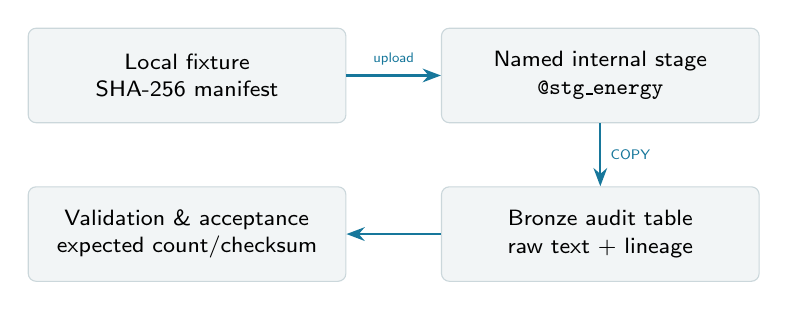
\begin{tikzpicture}[>=Stealth,node distance=6mm, every node/.style={font=\sffamily\fontsize{8}{10}\selectfont},bx/.style={draw=thinrule,rounded corners=1mm,fill=papergray,align=center,text width=38mm,minimum height=12mm}]
\node[bx] (a) {Local fixture\\SHA-256 manifest};
\node[bx,right=12mm of a] (b) {Named internal stage\\\texttt{@stg\_energy}};
\node[bx,below=8mm of b] (c) {Bronze audit table\\raw text + lineage};
\node[bx,below=8mm of a] (d) {Validation \& acceptance\\expected count/checksum};
\draw[->,thick,steelblue](a)--node[above]{\tiny upload}(b);
\draw[->,thick,steelblue](b)--node[right]{\tiny COPY}(c);
\draw[->,thick,steelblue](c)--(d);
\end{tikzpicture}\par{\fontsize{8}{10}\selectfont\color{inkgray}Figure 5.2. The stage is a transport boundary, not proof of correctness.}\end{center}
\textbf{Operational distinction.} Snowflake-managed internal storage reduces the need to configure another cloud bucket for a small lab. In a larger organization, the external stage may fit an established landing zone and independent retention policy. Both approaches still need an access audit, naming standard, encryption review, lifecycle rules and predictable cleanup.
\newpage
% page 84
\topic{5.3.2}{Storage integrations and object access}
An external stage delegates read access to a cloud location such as Amazon S3, Azure Blob Storage or Google Cloud Storage. Prefer Snowflake storage integrations and cloud-native trust policies over embedding long-lived access keys inside SQL. The integration has to be configured by a sufficiently privileged administrator and limited to expected locations. The object store's own policy must authorize the relevant Snowflake identity; the SQL object alone cannot grant access outside Snowflake.

\begin{lstlisting}[language=SQL,caption={External-stage shape; placeholders are not runnable credentials.}]
-- Administrator-reviewed example, NOT lab bootstrap:
CREATE STAGE energy_external
  URL = 's3://<approved-bucket>/energy/incoming/'
  STORAGE_INTEGRATION = <approved_integration>
  FILE_FORMAT = ff_energy_csv;
\end{lstlisting}
A secure integration is not merely ``the connection works.'' It must be narrow enough that a mistaken path cannot expose unrelated company objects. Review region, cross-cloud egress, object-store request charges, identity rotation and who may replace an object after the manifest is signed.

\topic{5.3.3}{Credential safety and file path conventions}
Treat object paths as stable identifiers with clear semantics. For example, a path grouped by publisher, metric and date helps operational navigation, but does \emph{not} replace the business observation key. Do not use a filename like \texttt{latest.csv} as a permanent identity: it can mean different bytes on two days.

\begin{whitebox}\textbf{Recommended landing layout}\par
\texttt{landing/source=fi\_energy\_demo/contract=v1/}\par
\texttt{\quad published\_date=2026-01-15/part-001.csv}\par
\texttt{manifest/source\_manifest.csv}\par
\texttt{quarantine/batch\_id=.../} (restricted access)\end{whitebox}
Authentication material belongs in approved secrets storage or short-lived identity providers; never in Git, notebooks, screenshots or example command history. For a demo, prefer an internal stage and local synthetic files. An external stage can be introduced once the permissions and cloud cost have been reviewed independently.

\textbf{Incident question.} What should happen when a file is replaced at the same path? The ingestion process must detect the checksum change, determine whether it is an authorized correction, and avoid assuming that a successful previous \texttt{COPY} makes the replacement safe.
\repo{P050: AWS storage-integration infrastructure example}{https://github.com/Snowflake-Labs/terraform-snowflake-storage-integration-aws}
\newpage
% page 85
\section*{5.4\quad Loading data with COPY INTO}
\topic{5.4.1}{COPY INTO with named formats}
\texttt{COPY INTO <table>} is the core SQL command for loading staged files into Snowflake. A reliable tutorial states the expected input and target shapes before running it. For this chapter each record has four fields: source code, metric, UTC interval and MWh value. Bronze accepts text as text so later validation can distinguish source defects from parser errors.

\begin{lstlisting}[language=SQL,caption={An auditable bronze target for unchanged source fields.}]
CREATE TABLE IF NOT EXISTS bronze_energy (
  source_code VARCHAR,
  metric VARCHAR,
  interval_text VARCHAR,
  value_text VARCHAR,
  source_file VARCHAR,
  source_row NUMBER,
  scanned_at TIMESTAMP_LTZ
);

COPY INTO bronze_energy (
  source_code, metric, interval_text, value_text,
  source_file, source_row, scanned_at
)
FROM (
  SELECT t.$1, t.$2, t.$3, t.$4,
         METADATA$FILENAME,
         METADATA$FILE_ROW_NUMBER,
         METADATA$START_SCAN_TIME
  FROM @stg_energy/ (FILE_FORMAT => ff_energy_csv) t
)
ON_ERROR = ABORT_STATEMENT;
\end{lstlisting}
This is a \emph{COPY transformation}: the select list combines file fields and Snowflake virtual metadata columns. Use an explicit column list to protect against accidental target-column order changes. The example assumes an existing authorized database and schema selected in the session; the companion project includes a complete scoped setup. The \texttt{METADATA\$START\_SCAN\_TIME} value records a scan boundary, not the publisher's original observation time [3].

\begin{insight}\textbf{Why text in bronze?}\par
If \texttt{value\_mwh} is initially loaded directly as \texttt{NUMBER}, a nonnumeric source token may abort the whole load or be skipped under a permissive error policy. Landing it as text makes the original value visible; a subsequent test can reject it with an attributable reason. This design is not a recommendation to skip validation indefinitely.\end{insight}
\repo{P006: Snowflake Northstar data engineering guide}{https://github.com/Snowflake-Labs/sfguide-snowflake-northstar-data-engineering}
\newpage
% page 86
\topic{5.4.2}{Duplicate-file loading behavior}
Snowflake keeps load metadata for file-based \texttt{COPY} into a table and normally avoids loading a previously recorded file again. That mechanism is useful for operational reruns, but it is not a universal exactly-once guarantee: files can be renamed, changed, staged in another way, or reprocessed after historical metadata becomes uncertain. The \texttt{FORCE=TRUE} option deliberately bypasses normal duplicate-file avoidance and can create duplicate rows [4].

\begin{center}\small\begin{tabularx}{\linewidth}{@{}p{40mm}X@{}}\toprule
Scenario & Expected engineering response\\\midrule
Same staged file, repeat COPY & Usually skipped while load status is known; inspect results\\
Same content, different path & Treat as possible duplicate at business-key layer\\
Changed file under same path & Compare content key and publisher revision contract\\
\texttt{FORCE=TRUE} & Explicit repair only, with pre/post reconciliation\\
Old file with uncertain history & Follow documented older-file policy; do not guess\\\bottomrule\end{tabularx}\end{center}
The older-file behavior is subtle. When load metadata is no longer decisive, Snowflake provides \texttt{LOAD\_UNCERTAIN\_FILES} and \texttt{FORCE} controls with different intents. Neither replaces a durable source manifest or a business-level deduplication rule [4]. An ingestion system should know which files it intended to process; the platform's recent history is supporting evidence, not its sole ledger.

\textbf{Failure scenario.} A scheduler crashes after Snowflake commits a load but before the orchestrator records success. Retrying exactly the same immutable file may be safely skipped by COPY's remembered status, but retrying a repackaged or renamed export may be processed again. The stable \emph{business key} (source, metric and interval) is therefore checked in the accepted layer. File-level identity and observation-level identity solve different problems.

\begin{insight}\textbf{Guardrail.}\par
Do not add \texttt{FORCE=TRUE} to a standard retry script. If a backfill genuinely requires reloading, isolate a batch, record its approval, choose a new versioned target or run a controlled reconciliation, and preserve the old manifest and load history.\end{insight}
\repo{P052: Community end-to-end Snowflake pipeline}{https://github.com/AvinashAnalytics/End-to-End-Snowflake-Data-Pipeline}
\newpage
% page 87
\topic{5.4.3}{Loading history and parsing options}
\texttt{COPY INTO} returns a result describing the files processed, rows parsed and loaded, and errors. Retain that statement's query ID and output as part of the orchestrator's batch record. A success message means the statement met its parser and load rules; it does not establish that the supplier provided every expected hour, used the correct unit or sent the latest revision.

For recent operations, Snowflake exposes an Information Schema \texttt{COPY\_HISTORY} table function covering the past 14 days; a separate Account Usage view has a broader, delayed history [5]. Access rights, object names and display latency must be reviewed before designing a production monitoring dashboard.

\begin{lstlisting}[language=SQL,caption={Investigate recently processed files; example scope.}]
SELECT file_name, status, row_count, row_parsed,
       error_count, last_load_time
FROM TABLE(INFORMATION_SCHEMA.COPY_HISTORY(
  TABLE_NAME => 'BRONZE_ENERGY',
  START_TIME => DATEADD('day', -1, CURRENT_TIMESTAMP())
))
ORDER BY last_load_time DESC;
\end{lstlisting}
A meaningful \emph{copy reconciliation} compares the expected files in the approved source manifest, the files that the load history reports, and the file/row counts actually present in the bronze table. These can disagree for legitimate reasons: a loaded file can have no valid business rows; a repeated file can be skipped; and an infrastructure failure can occur after the last file was committed but before the application received the result.

\begin{whitebox}\textbf{What to capture per ingestion attempt}\par
\texttt{batch\_id} and immutable manifest version; source/publisher; expected files, expected byte sizes and SHA-256; current Snowflake role/warehouse; started/completed UTC times; query ID; copy status; rows parsed/loaded; rejected rows; run result; a pointer to preserved logs.\end{whitebox}
\textbf{Performance warning.} Staging tens of thousands of tiny files can impose overhead even if their combined bytes are modest. Conversely, one extremely large compressed CSV can limit throughput for some parsing configurations. Choose file sizes using measured work with the real workload, not a universal number from a blog. Remember that \texttt{COPY\_HISTORY} is not a permanent substitute for an organization-owned audit ledger [4,5].

\textbf{Verification.} After loading two immutable files, identify their filenames, expected line counts, the \texttt{COPY} query ID and how you will prove whether a second invocation added any rows. Record data and control-plane timestamps in UTC.
\newpage
% page 88
\section*{5.5\quad File validation and rejected-record handling}
\topic{5.5.1}{VALIDATION\_MODE and ON\_ERROR}
A parser can fail because a file is malformed; a business rule can fail even when the file parses perfectly. Test both independently. The \texttt{ON\_ERROR} COPY option controls what happens to rows or files with \emph{load-level} errors. \texttt{ABORT\_STATEMENT} gives this small bronze exercise an auditable all-or-nothing default; \texttt{CONTINUE} trades that property for partial progress [3,6].

\begin{lstlisting}[language=SQL,caption={Optional structural dry run for a four-column file.}]
-- Separate validation table with only source columns.
CREATE TEMP TABLE csv_shape_check (
  source_code VARCHAR, metric VARCHAR,
  interval_text VARCHAR, value_text VARCHAR
);
COPY INTO csv_shape_check
FROM @stg_energy
FILE_FORMAT = (FORMAT_NAME = ff_energy_csv)
VALIDATION_MODE = RETURN_ALL_ERRORS;
\end{lstlisting}
\textbf{Critical restriction:} Snowflake does \emph{not} support \texttt{VALIDATION\_MODE} in a \texttt{COPY} statement that uses a \texttt{SELECT} transformation (such as the provenance-enriched load on the preceding pages). Neither \texttt{VALIDATION\_MODE} nor the \texttt{VALIDATE} table function is a general semantic data-quality engine [3,6]. In the companion lab, the validation check is separate, and a second query checks accepted numbers, times, keys and source revisions.

\topic{5.5.2}{Rejected-record quarantine}
Keep a quarantine record with the raw row, file path, row number, reason code and check version. Suggested reason codes distinguish bad timestamps, nonnumeric MWh, unknown metrics and unexpected sources. Do not equate a negative number with corruption until the domain contract says whether signed net flows are legitimate.

\topic{5.5.3}{Actionable ingestion error reports}
A useful incident report says which batch failed, which rule rejected it, how many rows are affected and whether publication is blocked. It includes a small redacted sample, a reproducible fixture and the relevant query ID. Alerting on \emph{rejected rows divided by evaluated rows} helps distinguish a one-off defect from a schema-wide change. Source credentials and personal data never belong in the error report.
\repo{P053: Data engineering with CoCo}{https://github.com/Snowflake-Labs/sfguide-data-engineering-with-coco}
\newpage
% page 89
\section*{5.6\quad Schema evolution, metadata, and provenance}
\topic{5.6.1}{Source-file and ingestion timestamp metadata}
Metadata transforms a disconnected row into an attributable observation. A bronze table should answer at least three questions: which file supplied this value, where was it in that file, and when did Snowflake read it? Snowflake exposes virtual filename, file-row-number, content-key and scan-start-time fields for supported staged-file workflows [7]. Their exact SQL names appear in the example below.

\begin{lstlisting}[language=SQL,caption={Preview row identity and staged-file metadata.}]
SELECT METADATA$FILENAME AS source_file,
       METADATA$FILE_ROW_NUMBER AS source_row,
       METADATA$FILE_CONTENT_KEY AS content_key,
       METADATA$START_SCAN_TIME AS scanned_at,
       t.$1 AS source_code,
       t.$4 AS value_text
FROM @stg_energy (FILE_FORMAT => ff_energy_csv) t;
\end{lstlisting}
Do not confuse \texttt{FILE\_CONTENT\_KEY}, a Snowflake metadata value, with the SHA-256 calculated by a local Python manifest generator. They answer related but not necessarily identical questions, and should not be assumed comparable or interchangeable without an explicit contract. The \texttt{START\_SCAN\_TIME} value is a warehouse observation, not a guarantee of when a publisher produced the original file.

\begin{center}\small\begin{tabularx}{\linewidth}{@{}p{35mm}X@{}}\toprule
Field & What it actually establishes\\\midrule
Event time & Time interval represented by source data\\
Published/revised at & Publisher claim, if captured independently\\
Retrieved at & When our downloader received the bytes\\
Staged at & When the client placed the object in the stage\\
Scanned at & Snowflake stage-file scan timestamp\\
Accepted at & Time a semantic quality gate accepted a version\\\bottomrule\end{tabularx}\end{center}
Preserving a single generic \texttt{created\_at} timestamp sacrifices this distinction. If a regulator or analyst asks why an energy total changed, a complete evidence chain includes the original file, the publisher's revision, the ingestion job, and the acceptance decision. This is more important than any one cloud feature.
\newpage
% page 90
\topic{5.6.2}{Schema drift and versioned contracts}
A schema can change syntactically (new field, renamed column, reordered CSV), semantically (MWh becomes kWh), or operationally (the publisher stops sending weekend files). A naive schema-evolution setting addresses only a subset of those changes. For production, version both the \emph{expected data contract} and the \emph{mapping code}; record the contract version with each batch's manifest.

\begin{center}\small\begin{tabularx}{\linewidth}{@{}p{25mm}p{42mm}X@{}}\toprule
Change & Recommended initial action & Reason\\\midrule
Added optional field & Review and version mapping & Might change business meaning\\
Renamed identifier & Quarantine / block & Breaks business-key semantics\\
Unit change & Block until mapped & Can corrupt totals silently\\
Column reorder & Fail positional header test & Shifts values across fields\\
Long source outage & Publish stale-state alert & Freshness SLO at risk\\\bottomrule\end{tabularx}\end{center}
Snowflake provides schema inference and automatic table schema evolution for supported load patterns, subject to configuration and privileges. Automatic schema evolution requires a table setting such as \texttt{ENABLE\_SCHEMA\_EVOLUTION}, column-name matching in the load, and an appropriate privilege; for CSV matching, header parsing and other parser settings matter [8]. These capabilities are not active by default in this deliberately narrow bronze load, and enabling them does \emph{not} make unreviewed changes safe.

\begin{insight}\textbf{Decision: evolve or hold?}\par
An added optional source description may be compatible with a contract update. A newly nullable key, changed time zone or altered unit cannot be accepted as a harmless extra column. Whenever a change could alter the meaning of an already-published metric, hold publication, preserve the new raw file, and require an explicit mapping version.\end{insight}
For a small teaching case, the companion Python validator checks the exact header and number of columns before upload. A separate semantic rule evaluates timestamps, metric codes and values after the bronze load. Readers can therefore distinguish a change in file \emph{shape} from a change in \emph{meaning}.

\textbf{Independent check.} Imagine the new export adds \texttt{source\_timezone} but retains timestamps in UTC. Does the current contract still mean the same thing? Possibly---provided the new field does not change the definition of \texttt{interval\_start\_utc}. Now imagine those timestamps silently switch to Helsinki local time. A shape-only test passes; a data-contract review must fail.
\newpage
% page 91
\topic{5.6.3}{Auditable provenance of transformed records}
Provenance is a chain of evidence rather than a note attached to a dashboard. A credible pipeline can trace a published result backward through an accepted observation, its selection among revisions, the bronze row, the staged file, and the source manifest. At each transition, the system should name the transformation and the invariant it preserved.

\begin{center}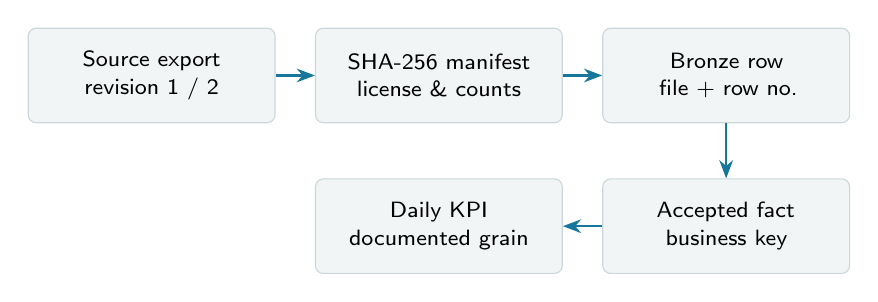
\begin{tikzpicture}[>=Stealth, every node/.style={font=\sffamily\fontsize{8.3}{10}\selectfont}, node distance=5mm, bx/.style={draw=thinrule,rounded corners=1mm,fill=papergray,text width=29mm,minimum height=12mm,align=center}]
\node[bx] (a) {Source export\\revision 1 / 2};
\node[bx,right=5mm of a] (b) {SHA-256 manifest\\license \& counts};
\node[bx,right=5mm of b] (c) {Bronze row\\file + row no.};
\node[bx,below=7mm of c] (d) {Accepted fact\\business key};
\node[bx,left=5mm of d] (e) {Daily KPI\\documented grain};
\draw[->,thick,steelblue](a)--(b);\draw[->,thick,steelblue](b)--(c);\draw[->,thick,steelblue](c)--(d);\draw[->,thick,steelblue](d)--(e);
\end{tikzpicture}\par{\fontsize{8}{10}\selectfont\color{inkgray}Figure 5.3. Traceability follows the selected revision into the reporting model.}\end{center}
A candidate load can pass its parser checks but fail the acceptance rule because the values are inconsistent with domain expectations. Retain both decisions: \emph{loaded into bronze} and \emph{accepted for analysis}. If a record is superseded, keep the earlier row traceable and mark the winner in a separate derived layer or documented view. Destroying revisions makes both reproducibility and incident investigation harder.

A practical source manifest has a stable batch ID, relative filename, SHA-256 digest, byte count, expected data rows, source revision, publisher and retrieval timestamps, contract version and source URL. A warehouse load ledger adds the COPY query ID, loaded count and status. Tie the two with a batch key rather than assuming the file name remains globally unique forever.

\begin{whitebox}\textbf{Data-lineage acceptance question}\par
For the national generation KPI displayed at \texttt{2026-01-15 01:00 UTC}, can you identify the source codes included, the accepted revision for each source, each staged file and the reason that an earlier reading was superseded? If the answer requires checking an engineer's private laptop, the publication process is not auditable.\end{whitebox}
\textbf{Design trade-off.} Keeping immutable source files has storage and retention costs, but can be significantly cheaper than explaining an irreproducible report. Apply a documented retention policy consistent with contracts and applicable data-protection duties; do not retain sensitive information merely because storage is easy.
\repo{P047: API source enrichment and provenance}{https://github.com/Snowflake-Labs/sfguide-getting-started-with-api-enrichment-framework}
\newpage
% page 92
\section*{5.7\quad Idempotency, deduplication, and load auditing}
\topic{5.7.1}{Exactly-once expectations versus practical idempotency}
Exactly-once is often used casually to mean ``my job can run twice without creating an incorrect result.'' That is a useful business objective, but it is not achieved solely by file-level COPY history. A stronger, testable invariant is: \emph{given the same approved manifest and source revisions, running the acceptance pipeline again produces the same set of accepted business keys and values}. This property is idempotency at the reporting boundary.

\topic{5.7.2}{Detecting duplicates and replayed loads}
Define the business key before removing duplicates. Our exercise uses \texttt{(source\_code, metric, interval\_start\_utc)}; a revision is a new candidate for the \emph{same} observation, not a seventh independent hour. The accepted result must choose the authorized highest revision deterministically. Sorting by arbitrary ingestion timestamp is insufficient if delayed files arrive out of order.

\begin{lstlisting}[language=SQL,caption={Find repeated business observations before publication.}]
WITH parsed AS (
 SELECT source_code, metric, interval_text,
        TRY_TO_DECIMAL(value_text,18,3) AS mwh
 FROM bronze_energy
)
SELECT source_code, metric, interval_text,
       COUNT(*) AS candidate_count
FROM parsed
GROUP BY source_code, metric, interval_text
HAVING COUNT(*) > 1;
\end{lstlisting}
This query detects multiple candidates; it does not decide which wins. The versioned manifest supplies publisher revision order; the acceptance transformation applies that order before aggregation. When a source lacks an explicit revision number, write a defensible tie-breaking policy and flag ambiguity rather than silently choosing the most convenient value.

\topic{5.7.3}{Audit identifiers and reconciliation checks}
\textbf{Three invariants:} (1) uploaded file count equals the approved manifest count; (2) bronze row count matches source rows plus any explicitly recorded partial-load deviations; (3) accepted business keys are unique, and their measure totals match the independently calculated fixture expectation. In the synthetic case used below, eight physical records contain one malformed value and one superseded revision: six current observations sum to \textbf{97.500 MWh}. These figures come from the companion fixture, not from a Finnish energy authority.
\repo{P043: Retail data-engineering pipeline reference}{https://github.com/Snowflake-Labs/sfguide-building-retail-analytics-de-pipeline}
\newpage
% page 93
\section*{5.8\quad Python-assisted batch ingestion}
\topic{5.8.1}{Python scripts for retrieval and staging}
Python is a useful orchestration boundary when a publisher exposes an HTTP API but not a Snowflake-native export. Keep it small: fetch or open a source file, validate its declared structure, calculate a checksum, write an immutable manifest, upload via an authorized client, and invoke a reviewed load. Do not embed data-cleaning surprises inside an ``easy'' helper function. The offline fixture uses only Python's standard library and needs no credentials.

\begin{lstlisting}[language=Python,caption={Core idea: a local file identity is byte-based.}]
import hashlib
from pathlib import Path

def sha256_file(path: Path) -> str:
    digest = hashlib.sha256()
    with path.open('rb') as stream:
        for chunk in iter(lambda: stream.read(1 << 20), b''):
            digest.update(chunk)
    return digest.hexdigest()
\end{lstlisting}
\topic{5.8.2}{Batching, retry/backoff, and rate limits}
HTTP download code should classify failures. A 401 or 403 usually requires a credential or authorization fix; a 429 calls for rate-limit handling; a transient 5xx might be retried with backoff and jitter. Set connect/read timeouts, a maximum attempt count and a maximum elapsed time. Respect the provider's \texttt{Retry-After} header where relevant. Resume only when the protocol and file identity make partial downloads safe; otherwise discard the incomplete file and start a new temporary download.

\topic{5.8.3}{Secret handling and idempotent invocations}
Promote a temporary file to its immutable, checksum-named destination only after integrity checks pass. A manifest update should be atomic from the orchestration perspective; publish it only after all listed files are present. Keep tokens in a secrets manager or narrowly scoped environment variables, never in the dataset, logs or repository. Restrict local staging permissions.

\begin{insight}\textbf{The retry trap.}\par
Retrying a GET request may download the same logical revision twice under different local filenames. If those filenames become new staged objects, Snowflake file-level duplicate detection may not recognize a repeated business event. Always reconcile the publisher revision ID or stable business key independently of local file naming.\end{insight}
\textbf{Hands-on task.} Run \texttt{python validate\_fixture.py}. Change one CSV header, then rerun. The test must fail before any upload. Restore the header, set a value to \texttt{N/A}, and observe structural success but semantic quarantine.
\repo{P054: AWS-to-Snowflake batch ETL example}{https://github.com/camposvinicius/aws-snowflake-etl}
\newpage
% page 94
\section*{5.9\quad Recovery procedures and ingestion monitoring}
\topic{5.9.1}{Recovery point selection and reprocessing}
A recoverable ingestion process knows the last \emph{approved manifest}, not merely the timestamp of the last scheduler success. On failure, establish whether the source was retrieved, the bytes staged, the copy committed and the acceptance output published. Retrying every step blindly can be wasteful or unsafe; a partial run should resume from the most recent verified boundary.

\begin{center}\small\begin{tabularx}{\linewidth}{@{}p{34mm}X@{}}\toprule
Observed failure & First safe diagnostic\\\midrule
Source fetch timeout & Compare downloaded checksum, retry policy, publication ID\\
Upload incomplete & Check stage listing vs approved manifest\\
COPY aborted & Preserve query ID; examine parser error, do not force reload\\
Bronze loaded, audit missing & Query COPY history and target before retrying\\
Acceptance test fails & Hold gold publishing, inspect quarantine and revisions\\\bottomrule\end{tabularx}\end{center}
\topic{5.9.2}{Observability dashboards and alerts}
Track five independent indicators: expected versus arrived files, successful versus rejected rows, accepted-key uniqueness, data freshness, and estimated ingestion cost. Alerting must distinguish no new data from no new \emph{valid} data. A dashboard that updates despite a failed source contract is not proof of pipeline health. Use incident severity and operational ownership appropriate to the organization rather than inheriting a demo's arbitrary thresholds.

\topic{5.9.3}{Cleanup, retention, and operational handover}
Stop or suspend lab compute when finished, remove only disposable chapter-scoped objects after explicit review, and keep the evidence needed for a reproducible acceptance test. Do not issue unrestricted \texttt{REMOVE @stage} or \texttt{DROP DATABASE} commands in a shared environment. An operations handover should contain the source owner, schema contract version, runbook, escalation route, cost controls, backfill procedure and rollback trigger.

\begin{whitebox}\textbf{Recovery decision checklist}\par
Record the incident ID; manifest ID; approved file list; target bronze count before/after; relevant Snowflake query IDs; failed acceptance tests; selected replay approach; authorization for any forced reload; and a post-recovery comparison of the expected business-key set.\end{whitebox}
\repo{P055: Snowflake Alert Hub reference}{https://github.com/Snowflake-Labs/sfguide-alert-hub}
\newpage
% page 95
\section*{5.L\quad Guided lab: a trustworthy bronze ingest}
\topic{5.L.1}{Prerequisites, inputs, and cost guardrails}
This lab continues the same \emph{synthetic} Finnish-energy-themed fixture introduced in Chapter~4. It intentionally contains a source revision and an invalid value so that a passing parser is not confused with a passing data-quality gate. Input: \texttt{energy\_r1.csv} (six records), \texttt{energy\_r2.csv} (a later correction and one invalid reading), and an automatically generated \texttt{source\_manifest.csv}. Expected raw rows: eight; accepted unique observations: six; accepted total: \textbf{97.500 MWh}.

An optional cloud run requires a disposable database/schema already authorized by the user, a limited ingest role, a small warehouse with auto-suspend, and a named internal stage. Assess credit charges before execution. The offline fixture verification requires no Snowflake account and no paid API calls. Never use production credentials or \texttt{ACCOUNTADMIN} as an everyday lab role.

\topic{5.L.2}{Procedure and selected code}
\textbf{Step 1:} Generate and verify the manifest before uploading; assert the header, row counts, file hashes and revision order. \textbf{Step 2:} Create the named CSV format, stage and bronze table using \texttt{sql/file\_formats.sql} and \texttt{sql/load\_batch.sql}. \textbf{Step 3:} Use a supported client to \texttt{PUT} the two files to the stage, leaving the immutable names unchanged. \textbf{Step 4:} Run the transformed \texttt{COPY} once; preserve its output and query ID. \textbf{Step 5:} Run quality queries, build the authorized revision selection and compare expected against actual.

\begin{lstlisting}[language=SQL,caption={The essential reconciliation: physical vs accepted rows.}]
SELECT COUNT(*) AS bronze_rows,
       COUNT(DISTINCT source_file) AS files_seen
FROM bronze_energy;
-- Expected after one successful copy: 8 rows, 2 files.

SELECT COUNT(*) AS invalid_numeric_rows
FROM bronze_energy
WHERE TRY_TO_DECIMAL(value_text,18,3) IS NULL;
-- Expected: 1 invalid numeric row in the fixture.
\end{lstlisting}
\textbf{Step 6:} Rerun the same \texttt{COPY} \emph{without} \texttt{FORCE}; inspect returned status and count changes. If the status is uncertain, stop rather than making repeated exploratory writes. \textbf{Step 7:} Confirm that the accepted layer chooses the revised solar value of 13.000 instead of the older 12.500. The manifest's revision order is authoritative for this synthetic exercise.

\begin{insight}\textbf{Evidence requirement.}\par
A screenshot of ``query completed'' is not a test. Preserve the input manifest, COPY query ID, target counts, rejected-record report, deterministic revision rule and the six accepted business keys. The companion archive includes an offline validator and expected results.\end{insight}
\newpage
% page 96
\topic{5.L.3}{Expected results, failure diagnosis, and cleanup}
The synthetic fixture produces a reproducible acceptance story: \textbf{two} unique files, \textbf{eight} physically loaded rows, \textbf{one} invalid numeric reading, \textbf{one} superseded revision, \textbf{six} accepted source/hour observations, and \textbf{97.500 MWh} across those accepted observations. These are fixture-derived assertions, not a claim that an actual Snowflake account was used in preparing the manuscript. A cloud reviewer should run the same queries in a clean account and save the real COPY results before release.

\textbf{If the counts differ, investigate in order:} (1) manifest file name/hash and record count; (2) stage contents and CSV parser; (3) copy history and query ID; (4) raw bronze row identity; (5) invalid timestamp/numeric rule; (6) source-revision precedence; (7) group-by business grain. Do not start by changing \texttt{FORCE} or removing duplicate rows with a blind \texttt{DISTINCT}. The lab's cleanup file contains \emph{commented} destructive statements only and an explicit warehouse-suspension reminder.

\topic{5.L.4}{Exercises, design review, and assessment}
\begin{enumerate}
\item \textbf{Foundation:} Explain why an 8-row bronze table does not imply eight valid energy observations. Name at least three distinct time fields in an ingestion ledger.
\item \textbf{Practitioner:} Introduce a third revision to one observation. Modify the manifest and test so the accepted count remains six, while the total reflects exactly the authorized replacement value.
\item \textbf{Architecture:} Compare one daily immutable CSV file with 24 small hourly files. Defend a choice using freshness, cost, recovery, source rights and operational complexity.
\end{enumerate}
\textbf{Scoring rubric (10 points).} Source contract and rights (2); parser/shape fidelity (2); manifest and provenance (2); deterministic acceptance (2); safe recovery and evidence (2). \textbf{Pass criterion:} at least 8/10 and no missing security or correctness gate.

\begin{whitebox}\textbf{Chapter 5 in one idea.}\quad Ingestion is a repeatable claim about which source bytes arrived, which records were accepted, and why a rerun will not rewrite the business story. Chapter~6 will extend this discipline to nested and semi-structured payloads.\end{whitebox}
{\fontsize{8.05}{9.9}\selectfont\textbf{Official reference notes (accessed 22 October 2026).}\par
[1] Snowflake, \href{https://docs.snowflake.com/en/sql-reference/sql/create-file-format}{CREATE FILE FORMAT}.\quad
[2] \href{https://docs.snowflake.com/en/sql-reference/sql/create-stage}{CREATE STAGE}.\quad
[3] \href{https://docs.snowflake.com/en/sql-reference/sql/copy-into-table}{COPY INTO table}.\quad
[4] \href{https://docs.snowflake.com/en/user-guide/data-load-considerations-load}{Loading considerations}.\quad
[5] \href{https://docs.snowflake.com/en/sql-reference/functions/copy_history}{COPY HISTORY}.\quad
[6] \href{https://docs.snowflake.com/en/user-guide/data-load-bulk-ts}{Bulk-load troubleshooting}.\quad
[7] \href{https://docs.snowflake.com/en/user-guide/querying-metadata}{Staged-file metadata}.\quad
[8] \href{https://docs.snowflake.com/en/user-guide/data-load-schema-evolution}{Schema evolution}.\par}
\end{document}
